%\documentclass[journal=jacsat]{achemso}

\documentclass[aps,prb,twocolumn,amsmath,amssymb,superscriptaddress,longbibliography]{revtex4-1}

%\documentclass[preprint,showpacs,preprintnumbers,amsmath,amssymb]{revtex4-1}
%\documentclass[twocolumn,showpacs,preprintnumbers,amsmath,amssymb]{revtex4}
% Some other (several out of many) possibilities
%\documentclass[preprint,aps]{revtex4}
%\documentclass[preprint,aps,draft]{revtex4}
%\documentclass[prb,amsmath,amssymb]{revtex4}% Physical Review B

\usepackage{tikz} %for adding axes labels to figures
\usepackage{graphicx}% Include figure files
\usepackage{epstopdf} %convert graphics
\usepackage{dcolumn}% Align table columns on decimal point
\usepackage{bm}% bold math
\usepackage{amsmath}% bold math
\usepackage{color}
\usepackage{booktabs}
%\usepackage[normalem]{ulem}
%\nofiles
\usetikzlibrary{positioning}

%shortcuts for sets of numbers
\newcommand{\Ns}{\mathbb{N}^{*}}
\newcommand{\N}{\mathbb{N}}
\newcommand{\Z}{\mathbb{Z}}
\newcommand{\Zs}{\mathbb{Z}^{*}}
\newcommand{\R}{\mathbb{R}}
\newcommand{\Rs}{\mathbb{R}^{*}}
\newcommand{\C}{\mathbb{C}}
\newcommand{\Cs}{\mathbb{C}^{*}}

\newcommand{\angstrom}{\text{\normalfont\AA}}
\newcommand\tab[1][1cm]{\hspace*{#1}} %tab shortcut

%\bibliographystyle{achemso}
%\bibliographystyle{unsrt}


%[COMPARE RAW NUMBERS; Elat (the bigger, the more ionic), Ect, etc.]


\begin{document}

\title{
%Using absolutely localized molecular orbitals for deeper physical insight into the nature of chemical bonding and linear-scaling calculations for condensed phase [binary] materials 
%Localized electrons (orbitals) in materials modeling
Using DFT to model $\text{TiO}_2$ nanoparticles
%Absolutely localized orbitals for density functional theory modeling of [binary] materials
}

\author{Nicolas Gastellu}
%\author{Yifei Shi}
\author{Rustam Z. Khaliullin}
\email{rustam.khaliullin@mcgill.ca}
\affiliation{Department of Chemistry, McGill University, 801 Sherbrooke St. West, Montreal, QC H3A 0B8, Canada}

\date{\today}

\begin{abstract} 

\end{abstract}

\maketitle
 

\section*{Introduction} 

\section*{Simulation details}

\subsection*{Classical MD}

\tab All classical MD simulations described in this work were ran in the $NpT$ ensemble, using the Matsui-Akaogi (MA) potential to model the interactions between pairs of atoms.
The MA potential was originally developed for classical MD simulations of the four main polytypes of crystalline $\text{TiO}_2$ and has been shown by previous studies to be the most adequate force field for predicting the structure and properties of its liquid and amorphous phases.
The MA potential describes the short-range interaction between atoms with a Buckingham potential and their long-range electrostatic interaction using the traditional Coulomb term:
\begin{equation}
V_{ij}(r) = f_{0}\cdot (B_i+B_j)\cdot\text{exp}\big(\frac{A_i + A_j - r}{B_i + B_j}\big) - \frac{C_{i}C_j}{r^6} + \frac{e\,Z_i\,Z_j}{4\pi\epsilon_0 r}\: ,
\end{equation}
where $r$ denotes the distance between the two interacting ions $i$ and $j$, $e$ is the elementary charge, $Z_i$ is the dimensionless ionic charge of ion $i$, $f_0$ is a standard force of 4.184$\,$kJ$\text{mol}^{-1}\angstrom^{-1}$, and $A_i$, $B_i$, and $C_i$ are parameters corresponding to $i$.
The numerical values of the constants listed above are given in table \ref{classpot}.

\begin{table}[]
\centering
\caption{Parameters used for evaluating the MA potentials.}
\label{classpot}
\
\begin{tabular}{ccccc}
\hline
Element & $Z$ ($|e|$) & $A$ ($\angstrom$) & $B$($\angstrom$) & $C$ $(\angstrom^3\text{kJ}^{1/2}\text{mol}^{-1/2})$ \\ \hline
Ti      & +2.196      & 1.1823            & 0.077            & 22.5                                                \\
O       & -1.098      & 1.6339            & 0.117            & 54.0                                                \\ \hline
\end{tabular}
\end{table}

\tab The atomic structures of the various $a-\text{TiO}_2$ nanoparticles described in this work were obtained in multiple steps.
We started by melting rutile ($r-\text{TiO}_2$) nanocrystals of 198, 390, 768, and 1842 atoms respectively whose structures were previously optimized at the BLYP/DZVP-GTH level of theory (using a plane wave energy cutoff of 2100 Ry) using classical MD in the $NPT$ ensemble with $T = 2000\,$K and $P_{\text{ext},0} = 0.0\,$Pa. 
We ran this first round of simulations for 40000 timesteps of $\Delta t = 0.5\,$fs.
The resulting melt was then cooled in three steps; classical MD simulations using the same potentials, ensemble, and number of steps were ran using $T = 1500\,$K,750$\,$K, and 300$\,$K successively, all with $\Delta t = 2.0\,$fs.
This process simulated the annealing of the melted nanocrystals into a glass which we then studied using Kohn-Sham DFT.

\tab Seeing as the MA potential was originally elaborated to describe the describe the structural properties of $r-\text{TiO}_2$, we also generated a set of conformations of a rutile lattice comprised of 72 atoms in the $NPT$ ensemble at $T = 300\,\text{K}$, using the same potential as described above.
Doing so provided us with energy values which we expect to be well correlated with the ones we obtain with DFT methods, thus giving us a reference data set to which we could compare the rest of our results.

\subsection{DFT calculations}

\tab Having obtained equilibriated atomic structures for nanoparticles of different sizes, we sampled 100 conformations from the last 40 ps of the last cooling run, at which point all four nanoparticles were in equilibrium with $T = 300\,\text{K}$ thermal bath.
We then ran single-point energy calculation using KS DFT at the PBE/DZVP level of theory, using a plane wave cutoff of 2000$\,$Ry.
We also ran similar DFT calculations the different configurations of the rutile lattice that we mentioned in the previous section.

%\tab Our results are discussed in the next section and plotted in figures 1-5, in which we plot the DFT energies of every configuration of a given nanoparticle vs the classically computed energies of those same configurations.
%We also added a $y = x$ line to help the reader any kind of correlation between both data sets. 

\section*{Results and discussion}

\tab For each nanoparticle, we compare the classically evaluated energy of every configuration against the energy obtained through a DFT calculation for that some configuration. 
We plot our results in figures 1-5.
This allows us to gauge the accuracy of MA forcefield; if the classical and quantum mechanical results are well correlated, then the purely classical representation of the forces in the nanoparticles is sufficiently accurate to discriminate between slight variations in a given system's configuration and can therefore be used to simulate this system nanoparticles instead of DFT, which is much more computationally expensive.


\begin{figure*}[htb]
\begin{tikzpicture}
  \node (img1)  {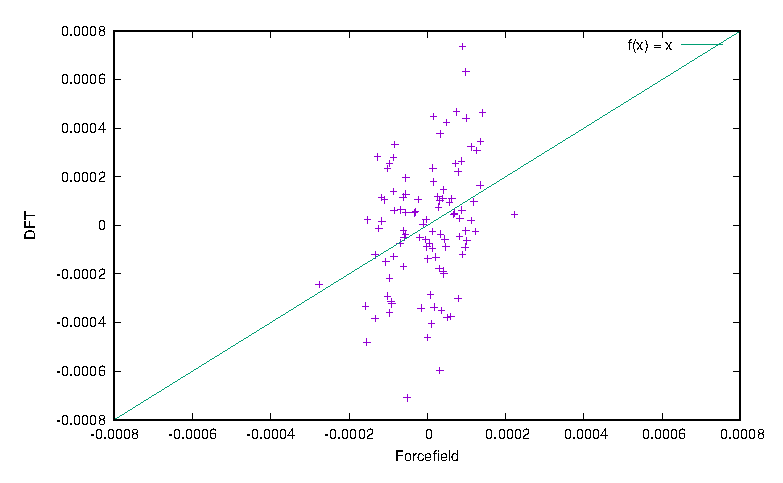
\includegraphics[scale=1.00]{./plots/nnp_198_scaled}};
  \node[below=of img1, node distance=0cm, yshift=1cm] {$E_{\text{classical} - \bar{E}_{\text{classical}}}$ (Ha)};
  \node[left=of img1, node distance=0cm, rotate=90, anchor=center,yshift=-0.7cm] {$E_{\text{DFT}} - \bar{E}_{\text{DFT}}$ (Ha)};
\end{tikzpicture}
\caption{DFT energy vs. classical energy (both shifted down by their average value) for 101 conformations of an $a-\text{TiO}_2$ nanoparticle with 198 atoms.}
\label{nnp_198}
\end{figure*}

\begin{figure*}[htb]
\begin{tikzpicture}
  \node (img1)  {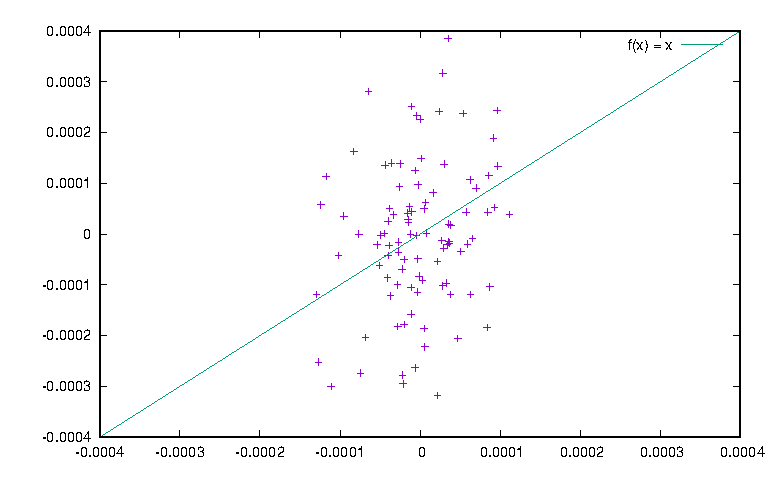
\includegraphics[scale=1.00]{./plots/nnp_390_scaled}};
  \node[below=of img1, node distance=0cm, yshift=1cm] {$E_{\text{classical} - \bar{E}_{\text{classical}}}$ (Ha)};
  \node[left=of img1, node distance=0cm, rotate=90, anchor=center,yshift=-0.7cm] {$E_{\text{DFT}} - \bar{E}_{\text{DFT}}$ (Ha)};
\end{tikzpicture}
\caption{DFT energy vs. classical energy (both shifted down by their average value) for 101 conformations of an $a-\text{TiO}_2$ nanoparticle with 390 atoms.}
\label{nnp_390}
\end{figure*}

\tab Comparing the energies obtained using classical MD and those calculated using DFT reveals that a description of the forces inside an $a-\text{TiO}_2$ nanoparticle using only the two-body MA potential is not precise enough to yield an accurate representation of its potential energy surface (PES) (with respect to its atoms' positions).
Indeed, plotting the energies yielded by both calculation methods reveals that DFT calculation methods are much more sensitive to a change in a given nanoparticle's atomic configuration than classical methods.


\begin{figure*}[htb]
\begin{tikzpicture}
  \node (img1)  {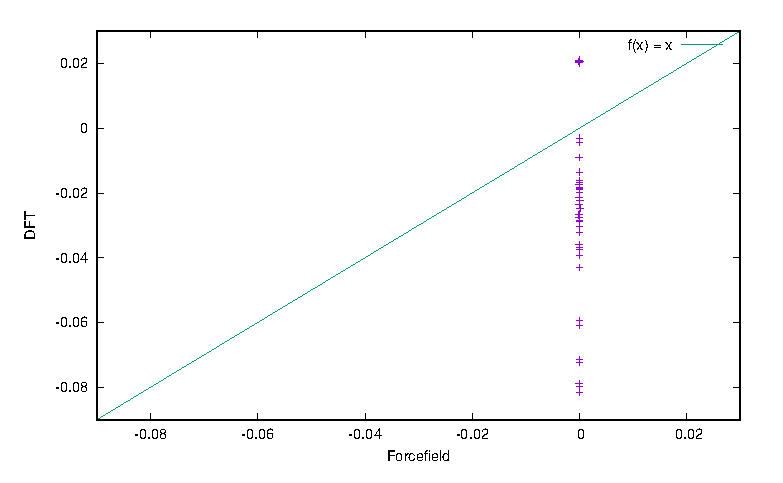
\includegraphics[scale=1.00]{./plots/nnp_768_fully_scaled}};
  \node[below=of img1, node distance=0cm, yshift=1cm] {$E_{\text{classical} - \bar{E}_{\text{classical}}}$ (Ha)};
  \node[left=of img1, node distance=0cm, rotate=90, anchor=center,yshift=-0.7cm] {$E_{\text{DFT}} - \bar{E}_{\text{DFT}}$ (Ha)};
\end{tikzpicture}
\caption{DFT energy vs. classical energy (both shifted down by their average value) for 101 conformations of an $a-\text{TiO}_2$ nanoparticle with 768 atoms.}
\label{nnp_768}
\end{figure*}

\tab The system for which this is the most obvious is the 768 atom nanoparticle, for which all classically evaluated energies lie within $\sim 10^{-4}\,\text{Ha}$ of each other, while the energies obtained usinq quantum mechanical methods vary by $\sim 10^{-1}\,\text{Ha}$.
While this effect is most dramatic for the 768 atom system, every other nanoparticle on which we ran similar calculations exhibit significant clustering of the energies obtained using the MA potential about their mean value, while their DFT energies spread out over a much larger interval\cite{realistic_nnp}.

\begin{figure*}[htb]
\begin{tikzpicture}
  \node (img1)  {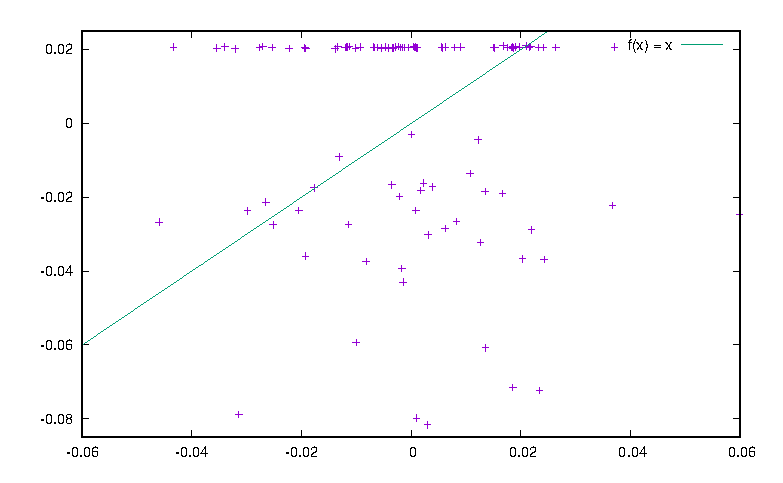
\includegraphics[scale=1.00]{./plots/nnp_768_dilated}};
  \node[below=of img1, node distance=0cm, yshift=1cm] {$500\cdot (E_{\text{classical} - \bar{E}_{\text{classical}})}$ (Ha)};
  \node[left=of img1, node distance=0cm, rotate=90, anchor=center,yshift=-0.7cm] {$E_{\text{DFT}} - \bar{E}_{\text{DFT}}$ (Ha)};
\end{tikzpicture}
\caption{Rescaled version of figure \ref{nnp_768}.}
\label{nnp_198}
\end{figure*}
    
\tab All four nanoparticles we ran these calculations exhibit weak correlation between the DFT-calculated energy values and the energies obtained using the MA potential. 
Even more surprisingly we find that the two sets of energy values of the different conformations of the rutile lattice were even less correlated than the ones obtained from the amorphous nanoparticles. 
Indeed, as can be seen in table \ref{stats}, our simulated rutile lattice yielded the lowest value of $\rho$ of all the systems we studied.
In light of this extremely low correlation, we obviously cannot consider our simulated $r-\text{TiO}_2$ lattice a reference system. 
However this is not overly problematic, it simply suggests that a purely classical two-body description of atomic interactions in $\text{TiO}_2$ in the amorphous or rutile phase is not sufficiently accurate to keep track of small changes in the system's configuration.
Moreover the small RMSE values we get for all systems (except the 768-atom nanoparticle) and the fact that all classically obtained energies for a given system are very close to each other suggest that they are still physically sound at a less precise level of analysis.
Indeed, if both sets of energy values for each system varied over intervals of similar sizes and yet remained as uncorrelated as we have observed them to be, then we would be in a position to question the validity of even trying to describe $\text{TiO}_2$ using only the MA potential in the first place.
However this is not the case; for every system all energies computed classically differ very little.
This is consistent with the fact that the atomic configurations from which such energies are computed were obtained from segments of our MD simulations where the system was already at equilibrium with its environment (i.e. the thermal bath) and thus did not vary greatly either.
The contrast between the highly clustered classical values and the much more spread out quantum values could therefore suggest that the quantum description of $\text{TiO}_2$ is much more sensitive to changes in the system's conformational changes while using the MA potential cannot meaningfully register such changes yet still provides an internally consistent and physically viable picture of the system.
[\textbf{Maybe: } This interpretation of our results is further corroborated by the higher $\rho$ values in smaller systems.] 

\begin{table*}[]
\begin{tabular}{c|c|c|c|c|c}
System & $a-\text{TiO}_2$ (198 atoms) & $a-\text{TiO}_2$ (390 atoms) & $a-\text{TiO}_2$ (768 atoms) & $a-\text{TiO}_2$ (1842 atoms) & $r-\text{TiO}_2$ (72 atoms) \\ \hline
$\rho$ & 0.3066474                    & 0.3497706                    & -0.0496755                   & TBC                           & 0.0141203                   \\
RMSE   & 0.0486056                    & 0.0628487                    & 22.21090                     & TBC                           & 0.0518275                   \\
\end{tabular}
\label{stats}
\caption{Pearson correlation coefficient $\rho$ and RMSE between the energy values obtained through DFT and those obtained using the two-body MA potential on various configurations of different systems.}
\end{table*}

\tab Having observed that DFT calculations are necessary to properly sample from an $a-\text{TiO}_2$ nanoparticle's PES, we are now faced with the problem posed by the computing power necessary to run such calculations on large systems (i.e. nanoparticles containing more than $\sim\,$1000 atoms).
Seeing as computational expense is one of DFT's main drawbacks, a number of optimisation schemes have been proposed over the years to reduce both the amount of memory and the time necessary to run such calculations.
Among them, we focus our attention to the absolutely localised molecular orbitals (ALMO) method which partitions the system being simulated into smaller fragments (usually these are the individual atoms or molecules that compose it) and runs traditional DFT on each fragment in parallel.
This has the advantage of having a runtime that scales linearly with the number of fragments for large systems.
Seeing as ALMO DFT makes a number of large DFT calculations much more feasible, we decide to test its accuracy on our various $a-\text{TiO}_2$ nanoparticles.
As before, we evaluate the accuracy of the ALMO DFT method by comparing the energy it outputs for a given configuration of a nanoparticle with the energy obtained through classical DFT.  

\section*{Conclusions} 



\textbf{Acknowledgments.} The research was funded by the Natural Sciences and Engineering Research Council of Canada through the Discovery Grant. The authors are grateful to Compute Canada and McGill HPC Centre for computer time.

%\textbf{Supporting Information}
%Calculated radial distribution functions of liquid water, comparison of timing benchmarks for the DZVP and TZV2P basis sets, timing benchmarks for systems containing 32,768 water molecules, timing benchmarks for the Kohn-Sham matrix build. This material is available free of charge via the Internet at http://pubs.acs.org.

\bibliography{tio2_nnp}




\end{document}
